\documentclass[a4paper,10pt,titlepage]{article}
% Språk och encodings
\usepackage[swedish,english]{babel}
\usepackage[T1]{fontenc}
\usepackage[utf8]{inputenc}
\usepackage[fixlanguage]{babelbib}
% Images and floats
\usepackage{graphicx}
\usepackage{wrapfig}
\usepackage{float}
% Clear type + Sans-serif font
\usepackage{lmodern}
\renewcommand{\familydefault}{\sfdefault}
% Avancerade tabeller
\usepackage{tabularx}
\usepackage{multirow}
\usepackage{booktabs}
% Matte
\usepackage{amsmath, amsthm, amssymb}
% Algoritmer
\usepackage[ruled,vlined]{algorithm2e}
% Källkod
\usepackage{listings}
\lstset{
	showspaces = false,
	showstringspaces = false,
}
% Inkludera pdf-sidor
\usepackage{pdfpages}
% Länkar
\usepackage{color}
\definecolor{dark-blue}{rgb}{0, 0, 0.6}
\usepackage{hyperref}
\hypersetup{
  colorlinks=true,
  linkcolor=dark-blue,
  urlcolor=dark-blue
}
% Vettiga paragrafer
\setlength{\parindent}{0pt}
\setlength{\parskip}{2ex}

% Kommando för kommandorader
\newcommand{\cmdline}[1]{\mbox{\textbf{\texttt{> #1}}}}

% Kommandon för testfall
\usepackage{testcases}

% Sidhuvud/sidfot
\usepackage{fancyhdr}
\setlength{\headheight}{15pt}
\pagestyle{fancyplain}
\lfoot{Carl-Oscar Erneholm \\ 880422-0872 \\ coer@kth.se}
\rfoot{Martin Nycander \\ 881028-0076 \\ mnyc@kth.se}
\cfoot{Sida \thepage}

% Språk
\selectbiblanguage{swedish}
\selectlanguage{swedish}

% Titel
\title{Laborationsrapport 2 \\ Small-Shell v2.51 för UNIX}
\author{Carl-Oscar Erneholm \and Martin Nycander}
\date{\today}

\begin{document}

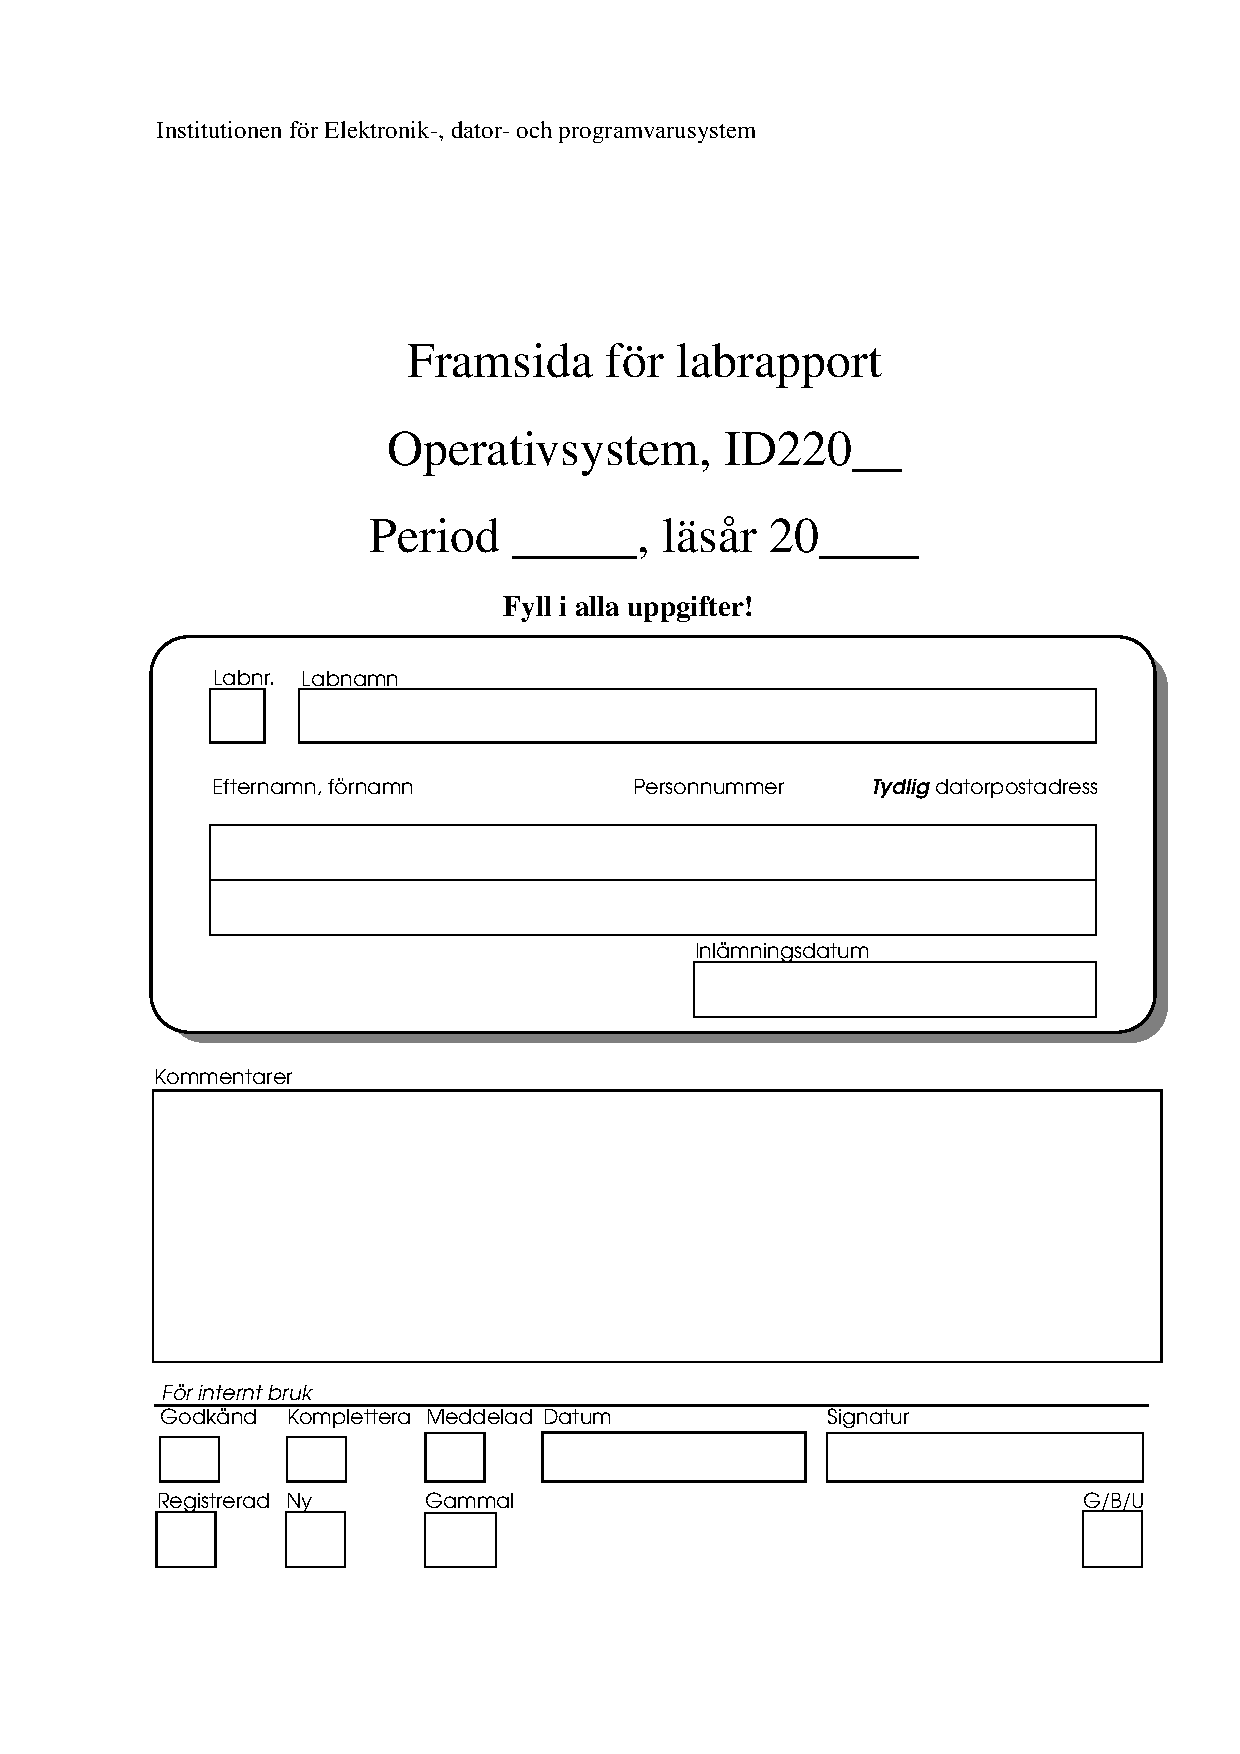
\includepdf[pages=-]{framsida.pdf}

\maketitle

\tableofcontents
\thispagestyle{empty}
\newpage
\setcounter{page}{1}
\section{Problembeskivning}

\subsection{Förberedelsefrågor}


\begin{enumerate}
	\item[1.] \textbf{\footnotesize Motivera varför det ofta är bra att exekvera kommandon i en separat process.}

	Om programmet krachar är det enklare att komma tillbaka till prompten och
    det blir lättare att implementera \verb!Ctrl+c! och \verb!Ctrl+z! eftersom
    shell processen kan lyssna efter input.

	\item[2.] \textbf{\footnotesize Vad händer om man inte i kommandotolken exekverar wait() för en barn-process som avslutas?}
	Barn-processen kommer finnas kvar som zombieprocess tills dess att shell
    programmet avslutas.
	\verb!//TODO!


	\item[3.] \textbf{\footnotesize Hur skall man utläsa SIGSEGV?}
	
	\verb!//TODO!


	\item[4.] \textbf{\footnotesize Varför kan man inte blockera SIGKILL?}
    För att man inte ska kunna skapa odödliga processer.


	\item[5.] \textbf{\footnotesize Hur skall man utläsa deklarationen void (*disp)(int))?}
	
    Det är en funktionspekare som pekar på en funktion som returnerar void och
    tar en int som parameter.


	\item[6.] \textbf{\footnotesize Vilket systemanrop använder sigset(3C) troligtvis för att installera en signalhanterare?}
	
	\verb!//TODO!


	\item[7.] \textbf{\footnotesize Hur gör man för att din kommandotolk inte skall termineras då en förgrundsprocess i den termineras med <Ctrl-c>?}
	
	\verb!//TODO!


	\item[8.] \textbf{\footnotesize Studera körningsexemplet nedan och förklara varför man inte har bytt “working directory” till /home/ds/robertr när man avslutat miniShell:et?}
	
	\verb!//TODO!

\end{enumerate}

\newpage
\section{Programbeskrivning}

\newpage
\section{Tester}

För att testa funktionaliten av vårat program har vi valt att köra följande kontrollerade tester:

\begin{testcase}{Start av förgrundsprocess}
	\prereq{\begin{checklist}
		\item Kommandotolken är startad.
		\item Programmet \texttt{echo} finns.
	\end{checklist}}
	\actions{
		\cmdline{echo "Test"}
	}
	\result{\begin{checklist}
			\item ``Test'' skrivs ut i kommandotolken.
			\item \texttt{echo} terminerar ordentligt (kontrollera med \cmdline{ps -aux}).
		\end{checklist}}
\end{testcase}

\begin{testcase}{Tomma strängen}
	\prereq{Kommandotolken är startad.}
	\actions{Ge ingen input, tryck bara enter.}
	\result{Kommandotolken kraschar inte.}
\end{testcase}

\begin{testcase}{Start av bakgrundsprocess}
	\prereq{\begin{checklist}
		\item Kommandotolken är startad.
		\item Programmet \texttt{sleep} finns.
		\item Programmet \texttt{echo} finns.
	\end{checklist}}
	\actions{\begin{actionlist}
		\item \cmdline{sleep 10\&}
		\item \cmdline{echo "Test"}
	\end{actionlist}
	}
	\result{\begin{checklist}
			\item Man behöver inte vänta 10 sekunder innan man får köra \cmdline{echo "Test"}
			\item ``Test'' skrivs ut i kommandotolken.
			\item Programmen terminerar ordentligt (kontrollera med \cmdline{ps -aux}).
		\end{checklist}}
\end{testcase}

\begin{testcase}{Bakgrundsprocesser och förgrundsprocesser}
	\prereq{\begin{checklist}
		\item Kommandotolken är startad.
		\item Programmet \texttt{sleep} finns.
	\end{checklist}}
	\actions{\begin{actionlist}
		\item \cmdline{sleep 5\&}
		\item \cmdline{sleep 10}
	\end{actionlist}
	}
	\result{\begin{checklist}
			\item Programmen terminerar i rätt ordning (först \cmdline{sleep \&}, sedan \cmdline{sleep 10}).
			\item Programmen terminerar ordentligt (kontrollera med \cmdline{ps -aux}).
		\end{checklist}}
\end{testcase}

\begin{testcase}{Avslutning med ``exit''}
	\prereq{Kommandotolken är startad.}
	\actions{\cmdline{./exit}}
	\result{\begin{checklist}
		\item Kommandotolken avslutas.
		\item Inga zombie-processer finns kvar (kontrollera med \cmdline{ps -aux}).
	\end{checklist}}
\end{testcase}

\begin{testcase}{Byte av arbetskatalog}
	\prereq{\begin{checklist}
		\item Kommandotolken är startad.
		\item Environmentvariabeln \texttt{HOME} är satt till ett känt värde.
	\end{checklist}}
	\actions{\begin{actionlist}
		\item Exekvera ``\cmdline{cd}''
		\item Exekvera ``\cmdline{pwd}'' och notera resultatet (1).
		\item Exekvera ``\cmdline{cd /etc}''
		\item Exekvera ``\cmdline{pwd}'' och notera resultatet (2).
		\item Exekvera ``\cmdline{cd .}''
		\item Exekvera ``\cmdline{pwd}'' och notera resultatet (3).
		\item Exekvera ``\cmdline{cd /åäö404}''
		\item Exekvera ``\cmdline{pwd}'' och notera resultatet (4).
		\item Exekvera ``\cmdline{cd.}''
		\item Exekvera ``\cmdline{pwd}'' och notera resultatet (5).
	\end{actionlist}}
	\result{\begin{checklist}
		\item Resultat 1, 3, 4 och 5 borde vara samma som värdet på \texttt{HOME}-variabeln.
		\item Resultat 2 borde vara ``/etc''.
	\end{checklist}}
\end{testcase}

\begin{testcase}{Informationsutskrifter}
	\prereq{\begin{checklist}
		\item Kommandotolken är startad.
		\item Programmet \texttt{sleep} finns.
	\end{checklist}}
	\actions{\cmdline{sleep 2}}
	\result{
		Följande information skrivs ut:
		\begin{checklist}
			\item Processid
			\item Att det är en förgrundsprocess.
			\item Att processen skapades och terminerades.
			\item Statistik över hur lång tid kommandot tog att genomföra.
		\end{checklist}
	}
\end{testcase}

\begin{testcase}{Terminering med Ctrl+c}
	\prereq{\begin{checklist}
		\item Kommandotolken är startad.
		\item Programmet \texttt{sleep} finns.
	\end{checklist}}
	\actions{\begin{actionlist}
		\item \cmdline{sleep 20}
		\item Avsluta exekveringen med \texttt{Ctrl+c} innan programmet avslutar sig själv.
	\end{actionlist}}
	\result{\begin{checklist}
		\item \texttt{sleep} avslutas (kontrollera med ps -aux).
		\item Kommandotolken avslutas \textbf{inte}.
	\end{checklist}}
\end{testcase}

\newpage
\section{Resultat}

Körning av ovanstående standardiserade testfall gav följande resultat.



\begin{testresults}{\today}
\end{testresults}

\newpage
\section{Labbutvärdering}


\newpage
\section{Källkod}

\lstset{tabsize=2}
\footnotesize{\lstinputlisting[language=C]{../program/minishell.c}}


\end{document}
